% Created by tikzDevice version 0.8.1 on 2015-11-17 11:43:51
% !TEX encoding = UTF-8 Unicode
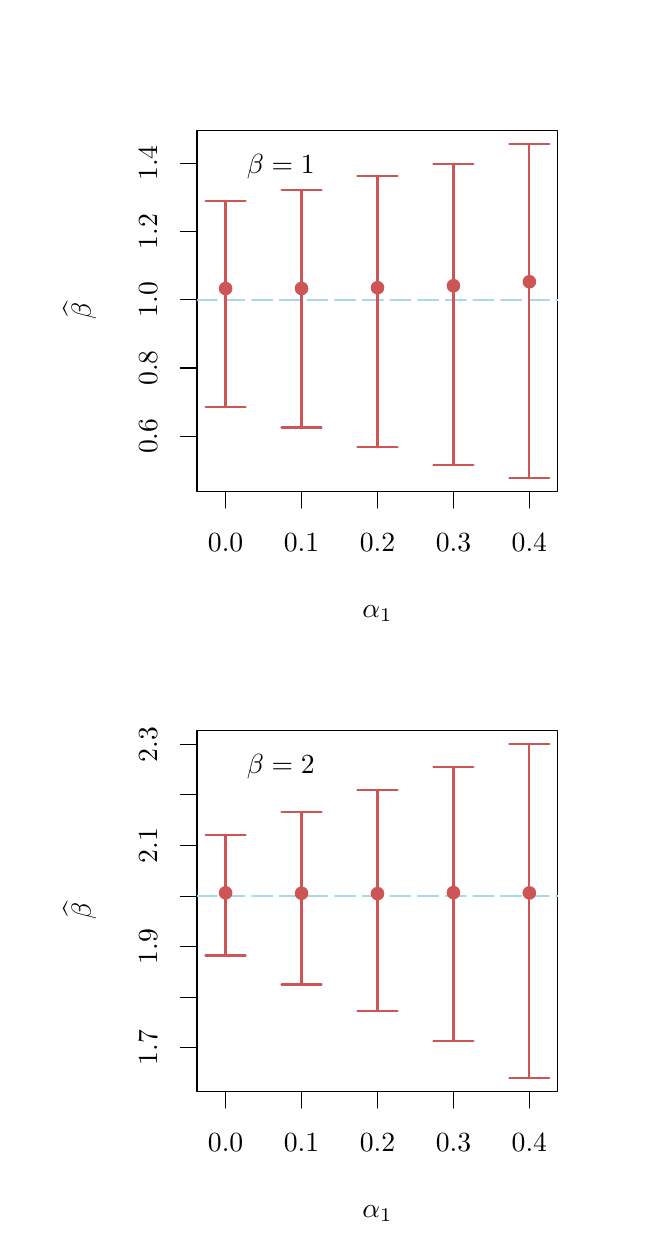
\begin{tikzpicture}[x=1pt,y=1pt]
\definecolor{fillColor}{RGB}{255,255,255}
\path[use as bounding box,fill=fillColor,fill opacity=0.00] (0,0) rectangle (216.81,433.62);
\begin{scope}
\path[clip] ( 61.20,266.01) rectangle (191.61,396.42);
\definecolor{drawColor}{RGB}{255,255,255}
\definecolor{fillColor}{RGB}{255,255,255}

\path[draw=drawColor,line width= 0.4pt,line join=round,line cap=round,fill=fillColor] ( 71.52,339.36) circle (  2.25);

\path[draw=drawColor,line width= 0.4pt,line join=round,line cap=round,fill=fillColor] ( 98.96,339.38) circle (  2.25);

\path[draw=drawColor,line width= 0.4pt,line join=round,line cap=round,fill=fillColor] (126.41,339.66) circle (  2.25);

\path[draw=drawColor,line width= 0.4pt,line join=round,line cap=round,fill=fillColor] (153.85,340.37) circle (  2.25);

\path[draw=drawColor,line width= 0.4pt,line join=round,line cap=round,fill=fillColor] (181.29,341.80) circle (  2.25);
\end{scope}
\begin{scope}
\path[clip] (  0.00,  0.00) rectangle (216.81,433.62);
\definecolor{drawColor}{RGB}{0,0,0}

\path[draw=drawColor,line width= 0.4pt,line join=round,line cap=round] ( 71.52,266.01) -- (181.29,266.01);

\path[draw=drawColor,line width= 0.4pt,line join=round,line cap=round] ( 71.52,266.01) -- ( 71.52,260.01);

\path[draw=drawColor,line width= 0.4pt,line join=round,line cap=round] ( 98.96,266.01) -- ( 98.96,260.01);

\path[draw=drawColor,line width= 0.4pt,line join=round,line cap=round] (126.41,266.01) -- (126.41,260.01);

\path[draw=drawColor,line width= 0.4pt,line join=round,line cap=round] (153.85,266.01) -- (153.85,260.01);

\path[draw=drawColor,line width= 0.4pt,line join=round,line cap=round] (181.29,266.01) -- (181.29,260.01);

\node[text=drawColor,anchor=base,inner sep=0pt, outer sep=0pt, scale=  1.00] at ( 71.52,244.41) {0.0};

\node[text=drawColor,anchor=base,inner sep=0pt, outer sep=0pt, scale=  1.00] at ( 98.96,244.41) {0.1};

\node[text=drawColor,anchor=base,inner sep=0pt, outer sep=0pt, scale=  1.00] at (126.41,244.41) {0.2};

\node[text=drawColor,anchor=base,inner sep=0pt, outer sep=0pt, scale=  1.00] at (153.85,244.41) {0.3};

\node[text=drawColor,anchor=base,inner sep=0pt, outer sep=0pt, scale=  1.00] at (181.29,244.41) {0.4};

\path[draw=drawColor,line width= 0.4pt,line join=round,line cap=round] ( 61.20,285.97) -- ( 61.20,384.68);

\path[draw=drawColor,line width= 0.4pt,line join=round,line cap=round] ( 61.20,285.97) -- ( 55.20,285.97);

\path[draw=drawColor,line width= 0.4pt,line join=round,line cap=round] ( 61.20,310.65) -- ( 55.20,310.65);

\path[draw=drawColor,line width= 0.4pt,line join=round,line cap=round] ( 61.20,335.32) -- ( 55.20,335.32);

\path[draw=drawColor,line width= 0.4pt,line join=round,line cap=round] ( 61.20,360.00) -- ( 55.20,360.00);

\path[draw=drawColor,line width= 0.4pt,line join=round,line cap=round] ( 61.20,384.68) -- ( 55.20,384.68);

\node[text=drawColor,rotate= 90.00,anchor=base,inner sep=0pt, outer sep=0pt, scale=  1.00] at ( 46.80,285.97) {0.6};

\node[text=drawColor,rotate= 90.00,anchor=base,inner sep=0pt, outer sep=0pt, scale=  1.00] at ( 46.80,310.65) {0.8};

\node[text=drawColor,rotate= 90.00,anchor=base,inner sep=0pt, outer sep=0pt, scale=  1.00] at ( 46.80,335.32) {1.0};

\node[text=drawColor,rotate= 90.00,anchor=base,inner sep=0pt, outer sep=0pt, scale=  1.00] at ( 46.80,360.00) {1.2};

\node[text=drawColor,rotate= 90.00,anchor=base,inner sep=0pt, outer sep=0pt, scale=  1.00] at ( 46.80,384.68) {1.4};

\path[draw=drawColor,line width= 0.4pt,line join=round,line cap=round] ( 61.20,266.01) --
	(191.61,266.01) --
	(191.61,396.42) --
	( 61.20,396.42) --
	( 61.20,266.01);
\end{scope}
\begin{scope}
\path[clip] (  0.00,216.81) rectangle (216.81,433.62);
\definecolor{drawColor}{RGB}{0,0,0}

\node[text=drawColor,anchor=base,inner sep=0pt, outer sep=0pt, scale=  1.00] at (126.41,220.41) {$\alpha_1$};

\node[text=drawColor,rotate= 90.00,anchor=base,inner sep=0pt, outer sep=0pt, scale=  1.00] at ( 22.80,331.22) {$\widehat{\beta}$};
\end{scope}
\begin{scope}
\path[clip] ( 61.20,266.01) rectangle (191.61,396.42);
\definecolor{drawColor}{RGB}{0,0,0}

\node[text=drawColor,anchor=base west,inner sep=0pt, outer sep=0pt, scale=  1.00] at ( 79.20,380.98) {$\beta=1$};
\definecolor{drawColor}{RGB}{173,216,230}

\path[draw=drawColor,line width= 0.8pt,dash pattern=on 7pt off 3pt ,line join=round,line cap=round] ( 61.20,335.32) -- (191.61,335.32);

\path[draw=drawColor,line width= 0.8pt,dash pattern=on 7pt off 3pt ,line join=round,line cap=round] ( 61.20,335.32) -- (191.61,335.32);

\path[draw=drawColor,line width= 0.8pt,dash pattern=on 7pt off 3pt ,line join=round,line cap=round] ( 61.20,335.32) -- (191.61,335.32);

\path[draw=drawColor,line width= 0.8pt,dash pattern=on 7pt off 3pt ,line join=round,line cap=round] ( 61.20,335.32) -- (191.61,335.32);

\path[draw=drawColor,line width= 0.8pt,dash pattern=on 7pt off 3pt ,line join=round,line cap=round] ( 61.20,335.32) -- (191.61,335.32);
\definecolor{drawColor}{RGB}{205,85,85}

\path[draw=drawColor,line width= 0.8pt,line join=round,line cap=round] ( 71.52,296.63) -- ( 71.52,370.87);

\path[draw=drawColor,line width= 0.8pt,line join=round,line cap=round] ( 64.29,296.63) --
	( 71.52,296.63) --
	( 78.75,296.63);

\path[draw=drawColor,line width= 0.8pt,line join=round,line cap=round] ( 78.75,370.87) --
	( 71.52,370.87) --
	( 64.29,370.87);

\path[draw=drawColor,line width= 0.8pt,line join=round,line cap=round] ( 98.96,289.16) -- ( 98.96,374.89);

\path[draw=drawColor,line width= 0.8pt,line join=round,line cap=round] ( 91.73,289.16) --
	( 98.96,289.16) --
	(106.19,289.16);

\path[draw=drawColor,line width= 0.8pt,line join=round,line cap=round] (106.19,374.89) --
	( 98.96,374.89) --
	( 91.73,374.89);

\path[draw=drawColor,line width= 0.8pt,line join=round,line cap=round] (126.41,281.97) -- (126.41,380.08);

\path[draw=drawColor,line width= 0.8pt,line join=round,line cap=round] (119.18,281.97) --
	(126.41,281.97) --
	(133.63,281.97);

\path[draw=drawColor,line width= 0.8pt,line join=round,line cap=round] (133.63,380.08) --
	(126.41,380.08) --
	(119.18,380.08);

\path[draw=drawColor,line width= 0.8pt,line join=round,line cap=round] (153.85,275.69) -- (153.85,384.26);

\path[draw=drawColor,line width= 0.8pt,line join=round,line cap=round] (146.62,275.69) --
	(153.85,275.69) --
	(161.08,275.69);

\path[draw=drawColor,line width= 0.8pt,line join=round,line cap=round] (161.08,384.26) --
	(153.85,384.26) --
	(146.62,384.26);

\path[draw=drawColor,line width= 0.8pt,line join=round,line cap=round] (181.29,270.84) -- (181.29,391.59);

\path[draw=drawColor,line width= 0.8pt,line join=round,line cap=round] (174.06,270.84) --
	(181.29,270.84) --
	(188.52,270.84);

\path[draw=drawColor,line width= 0.8pt,line join=round,line cap=round] (188.52,391.59) --
	(181.29,391.59) --
	(174.06,391.59);
\definecolor{fillColor}{RGB}{205,85,85}

\path[draw=drawColor,line width= 0.4pt,line join=round,line cap=round,fill=fillColor] ( 71.52,339.36) circle (  2.25);

\path[draw=drawColor,line width= 0.4pt,line join=round,line cap=round,fill=fillColor] ( 98.96,339.38) circle (  2.25);

\path[draw=drawColor,line width= 0.4pt,line join=round,line cap=round,fill=fillColor] (126.41,339.66) circle (  2.25);

\path[draw=drawColor,line width= 0.4pt,line join=round,line cap=round,fill=fillColor] (153.85,340.37) circle (  2.25);

\path[draw=drawColor,line width= 0.4pt,line join=round,line cap=round,fill=fillColor] (181.29,341.80) circle (  2.25);
\end{scope}
\begin{scope}
\path[clip] ( 61.20, 49.20) rectangle (191.61,179.61);
\definecolor{drawColor}{RGB}{255,255,255}
\definecolor{fillColor}{RGB}{255,255,255}

\path[draw=drawColor,line width= 0.4pt,line join=round,line cap=round,fill=fillColor] ( 71.52,120.99) circle (  2.25);

\path[draw=drawColor,line width= 0.4pt,line join=round,line cap=round,fill=fillColor] ( 98.96,120.84) circle (  2.25);

\path[draw=drawColor,line width= 0.4pt,line join=round,line cap=round,fill=fillColor] (126.41,120.71) circle (  2.25);

\path[draw=drawColor,line width= 0.4pt,line join=round,line cap=round,fill=fillColor] (153.85,121.08) circle (  2.25);

\path[draw=drawColor,line width= 0.4pt,line join=round,line cap=round,fill=fillColor] (181.29,120.97) circle (  2.25);
\end{scope}
\begin{scope}
\path[clip] (  0.00,  0.00) rectangle (216.81,433.62);
\definecolor{drawColor}{RGB}{0,0,0}

\path[draw=drawColor,line width= 0.4pt,line join=round,line cap=round] ( 71.52, 49.20) -- (181.29, 49.20);

\path[draw=drawColor,line width= 0.4pt,line join=round,line cap=round] ( 71.52, 49.20) -- ( 71.52, 43.20);

\path[draw=drawColor,line width= 0.4pt,line join=round,line cap=round] ( 98.96, 49.20) -- ( 98.96, 43.20);

\path[draw=drawColor,line width= 0.4pt,line join=round,line cap=round] (126.41, 49.20) -- (126.41, 43.20);

\path[draw=drawColor,line width= 0.4pt,line join=round,line cap=round] (153.85, 49.20) -- (153.85, 43.20);

\path[draw=drawColor,line width= 0.4pt,line join=round,line cap=round] (181.29, 49.20) -- (181.29, 43.20);

\node[text=drawColor,anchor=base,inner sep=0pt, outer sep=0pt, scale=  1.00] at ( 71.52, 27.60) {0.0};

\node[text=drawColor,anchor=base,inner sep=0pt, outer sep=0pt, scale=  1.00] at ( 98.96, 27.60) {0.1};

\node[text=drawColor,anchor=base,inner sep=0pt, outer sep=0pt, scale=  1.00] at (126.41, 27.60) {0.2};

\node[text=drawColor,anchor=base,inner sep=0pt, outer sep=0pt, scale=  1.00] at (153.85, 27.60) {0.3};

\node[text=drawColor,anchor=base,inner sep=0pt, outer sep=0pt, scale=  1.00] at (181.29, 27.60) {0.4};

\path[draw=drawColor,line width= 0.4pt,line join=round,line cap=round] ( 61.20, 65.00) -- ( 61.20,174.64);

\path[draw=drawColor,line width= 0.4pt,line join=round,line cap=round] ( 61.20, 65.00) -- ( 55.20, 65.00);

\path[draw=drawColor,line width= 0.4pt,line join=round,line cap=round] ( 61.20, 83.28) -- ( 55.20, 83.28);

\path[draw=drawColor,line width= 0.4pt,line join=round,line cap=round] ( 61.20,101.55) -- ( 55.20,101.55);

\path[draw=drawColor,line width= 0.4pt,line join=round,line cap=round] ( 61.20,119.82) -- ( 55.20,119.82);

\path[draw=drawColor,line width= 0.4pt,line join=round,line cap=round] ( 61.20,138.09) -- ( 55.20,138.09);

\path[draw=drawColor,line width= 0.4pt,line join=round,line cap=round] ( 61.20,156.37) -- ( 55.20,156.37);

\path[draw=drawColor,line width= 0.4pt,line join=round,line cap=round] ( 61.20,174.64) -- ( 55.20,174.64);

\node[text=drawColor,rotate= 90.00,anchor=base,inner sep=0pt, outer sep=0pt, scale=  1.00] at ( 46.80, 65.00) {1.7};

\node[text=drawColor,rotate= 90.00,anchor=base,inner sep=0pt, outer sep=0pt, scale=  1.00] at ( 46.80,101.55) {1.9};

\node[text=drawColor,rotate= 90.00,anchor=base,inner sep=0pt, outer sep=0pt, scale=  1.00] at ( 46.80,138.09) {2.1};

\node[text=drawColor,rotate= 90.00,anchor=base,inner sep=0pt, outer sep=0pt, scale=  1.00] at ( 46.80,174.64) {2.3};

\path[draw=drawColor,line width= 0.4pt,line join=round,line cap=round] ( 61.20, 49.20) --
	(191.61, 49.20) --
	(191.61,179.61) --
	( 61.20,179.61) --
	( 61.20, 49.20);
\end{scope}
\begin{scope}
\path[clip] (  0.00,  0.00) rectangle (216.81,216.81);
\definecolor{drawColor}{RGB}{0,0,0}

\node[text=drawColor,anchor=base,inner sep=0pt, outer sep=0pt, scale=  1.00] at (126.41,  3.60) {$\alpha_1$};

\node[text=drawColor,rotate= 90.00,anchor=base,inner sep=0pt, outer sep=0pt, scale=  1.00] at ( 22.80,114.40) {$\widehat{\beta}$};
\end{scope}
\begin{scope}
\path[clip] ( 61.20, 49.20) rectangle (191.61,179.61);
\definecolor{drawColor}{RGB}{0,0,0}

\node[text=drawColor,anchor=base west,inner sep=0pt, outer sep=0pt, scale=  1.00] at ( 79.20,164.17) {$\beta=2$};
\definecolor{drawColor}{RGB}{173,216,230}

\path[draw=drawColor,line width= 0.8pt,dash pattern=on 7pt off 3pt ,line join=round,line cap=round] ( 61.20,119.82) -- (191.61,119.82);

\path[draw=drawColor,line width= 0.8pt,dash pattern=on 7pt off 3pt ,line join=round,line cap=round] ( 61.20,119.82) -- (191.61,119.82);

\path[draw=drawColor,line width= 0.8pt,dash pattern=on 7pt off 3pt ,line join=round,line cap=round] ( 61.20,119.82) -- (191.61,119.82);

\path[draw=drawColor,line width= 0.8pt,dash pattern=on 7pt off 3pt ,line join=round,line cap=round] ( 61.20,119.82) -- (191.61,119.82);

\path[draw=drawColor,line width= 0.8pt,dash pattern=on 7pt off 3pt ,line join=round,line cap=round] ( 61.20,119.82) -- (191.61,119.82);
\definecolor{drawColor}{RGB}{205,85,85}

\path[draw=drawColor,line width= 0.8pt,line join=round,line cap=round] ( 71.52, 98.35) -- ( 71.52,141.99);

\path[draw=drawColor,line width= 0.8pt,line join=round,line cap=round] ( 64.29, 98.35) --
	( 71.52, 98.35) --
	( 78.75, 98.35);

\path[draw=drawColor,line width= 0.8pt,line join=round,line cap=round] ( 78.75,141.99) --
	( 71.52,141.99) --
	( 64.29,141.99);

\path[draw=drawColor,line width= 0.8pt,line join=round,line cap=round] ( 98.96, 87.86) -- ( 98.96,150.16);

\path[draw=drawColor,line width= 0.8pt,line join=round,line cap=round] ( 91.73, 87.86) --
	( 98.96, 87.86) --
	(106.19, 87.86);

\path[draw=drawColor,line width= 0.8pt,line join=round,line cap=round] (106.19,150.16) --
	( 98.96,150.16) --
	( 91.73,150.16);

\path[draw=drawColor,line width= 0.8pt,line join=round,line cap=round] (126.41, 78.25) -- (126.41,158.03);

\path[draw=drawColor,line width= 0.8pt,line join=round,line cap=round] (119.18, 78.25) --
	(126.41, 78.25) --
	(133.63, 78.25);

\path[draw=drawColor,line width= 0.8pt,line join=round,line cap=round] (133.63,158.03) --
	(126.41,158.03) --
	(119.18,158.03);

\path[draw=drawColor,line width= 0.8pt,line join=round,line cap=round] (153.85, 67.37) -- (153.85,166.48);

\path[draw=drawColor,line width= 0.8pt,line join=round,line cap=round] (146.62, 67.37) --
	(153.85, 67.37) --
	(161.08, 67.37);

\path[draw=drawColor,line width= 0.8pt,line join=round,line cap=round] (161.08,166.48) --
	(153.85,166.48) --
	(146.62,166.48);

\path[draw=drawColor,line width= 0.8pt,line join=round,line cap=round] (181.29, 54.03) -- (181.29,174.78);

\path[draw=drawColor,line width= 0.8pt,line join=round,line cap=round] (174.06, 54.03) --
	(181.29, 54.03) --
	(188.52, 54.03);

\path[draw=drawColor,line width= 0.8pt,line join=round,line cap=round] (188.52,174.78) --
	(181.29,174.78) --
	(174.06,174.78);
\definecolor{fillColor}{RGB}{205,85,85}

\path[draw=drawColor,line width= 0.4pt,line join=round,line cap=round,fill=fillColor] ( 71.52,120.99) circle (  2.25);

\path[draw=drawColor,line width= 0.4pt,line join=round,line cap=round,fill=fillColor] ( 98.96,120.84) circle (  2.25);

\path[draw=drawColor,line width= 0.4pt,line join=round,line cap=round,fill=fillColor] (126.41,120.71) circle (  2.25);

\path[draw=drawColor,line width= 0.4pt,line join=round,line cap=round,fill=fillColor] (153.85,121.08) circle (  2.25);

\path[draw=drawColor,line width= 0.4pt,line join=round,line cap=round,fill=fillColor] (181.29,120.97) circle (  2.25);
\end{scope}
\end{tikzpicture}
